%version of 02-28-20

\chapter{The hidden beauty of numbers}
\label{Appendix:Tetra}

Our first objective here is to show amazing hidden structures in integer expressions.
The second objective (the most important one) is to develop the reasoning path which leads to these results.
One of the hardest part while proving a mathematical result is how to develop the insights to use an appropriate \textit{tool} (method, picture, etc.).
Our purpose in this section is to help to deeply understand what to do facing a mathematical problem.


%%%%%%%%%%%%%%%%%%%
\section{Revisiting triangular numbers}

The $n$ triangular number is defined as the sum of the $n$th first integers.
It is denoted by $\Delta_n$.

$\Delta_n =  \sum_{k=1}^{n} k$

In chapter~\ref{ch:Summation}, we proved the expression of $\Delta_n$ by two methods.
\begin{itemize}
\item the \textit{trick} of Gauss that evidences an invariant: the sum of the $k$th term plus the $n-k+1$th one
is equal to $n+1$. 
\item using the Fubini's double counting principle, where the $k$th integer is represented by $k$ tokens.
Putting two collections of tokens organized as triangles leads to a rectangle whose surface is equal to $n.(n+1)$
\end{itemize}
We present below a figure that is an intermediate between both methods and that will serve as the basic principle for further investigations.
Like for Gauss' trick, the sum of each of the n rows is an invariant (see the last column of Fig.~\ref{fig:Tetrahedral2}). 
\begin{figure}[h]
\begin{center}
        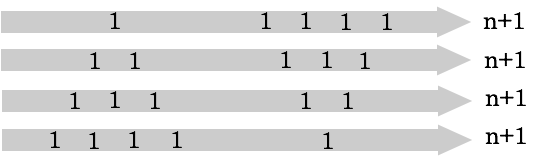
\includegraphics[scale=0.4]{FiguresArithmetic/appTetrahedral2}
        \caption{Computing $\Delta_n$ for $n=4$: two copies of a basic triangle pattern aligned in rows sum up to an invariant.}
        \label{fig:Tetrahedral2}
\end{center}
\end{figure}
$\Delta_n =  \sum_{k=1}^{n} k = \frac{1}{2}n.(n+1)$


%%%%%%%%%%%%%%%
\section{Tetrahedral numbers}
\label{sec:tetraedralNumbers}

We generalize in this section the previous result. The problem is to compute
the sum of the first triangular numbers, called tetrahedral numbers (the name comes from the 3 dimension representation, 
which has $4$ faces):

$\Theta_n =  \sum_{k=1}^{n} \Delta_k$

\subsection{A first look}

The natural way is to replace $\Delta_k$ by its value $\frac{n.(n+1)}{2}$ and to determine the expression
by arithmetic manipulations.

We left the verification to the readers, the expression is:

$\Theta_n =  \sum_{k=1}^{n} \Delta_k $

$=  \sum_{k=1}^{n} \frac{1}{2} (k^2 + k) $

$=  \frac{1}{2} (\sum_{k=1}^{n} k^2 + \sum_{k=1}^{n} k) $

Using expression~\ref{eq:sum-1-to-nsq} for the sum of squares:

$= \frac{1}{2} ( \frac{1}{3} n^3 + \frac{1}{2} n^2 + \frac{1}{6} n + \frac{1}{2} n^2 + \frac{1}{2} n )$

$= \frac{n.(n+1).(n+2)}{6}$

\medskip

Remark that this result can also easily been proved by recurrence as soon as the expression is known
(by guessing the expression).
We let the reader develop this type of proof. 


\subsection{Pictorial proof}

We detail now the proof using the double counting Fubini's principle.
Following this way, you should write the previous expression of the tetrahedral number in a developed form 
using a triangle shape like the one used in Fig.~\ref{fig:Tetrahedral2}
replacing the $1$'s by the successive integers.

A tetrahedral number is the sum of triangular numbers, and thus, it can be arranged as a triangle (see Fig.~\ref{fig:Tetrahedral3}).
As triangles have three sides, we have three ways to represent them (by rotating the sides) as shown in Fig.~\ref{fig:Tetrahedral1}..
Then, as before, the Fubini's principle will be used to sum up the successive rows.
The way to organize them is guided by the search of an invariant:
the sum of the elements over the rows of the three triangles is proportional to $n+2$.
\begin{figure}[h]
\begin{center}
        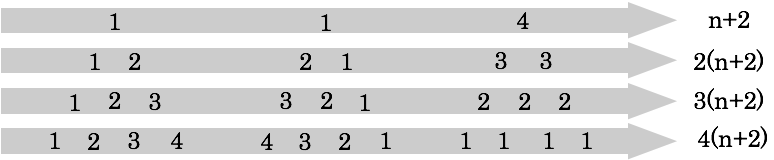
\includegraphics[scale=0.4]{FiguresArithmetic/appTetrahedral3}
        \caption{Basic pattern for computing $\Theta_n$ (for $n=4$).}
        \label{fig:Tetrahedral3}
\end{center}
\end{figure}
\begin{figure}[h]
\begin{center}
        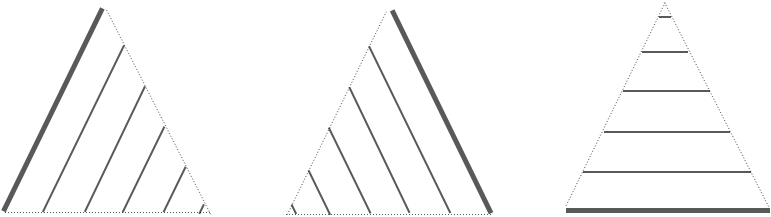
\includegraphics[scale=0.3]{FiguresArithmetic/appTetrahedral1}
        \caption{Schematic view of the three ways of organizing the triangles.
        The numbers are the same on each solid line, the bold one contains the $1$.}
        \label{fig:Tetrahedral1}
\end{center}
\end{figure}
\begin{figure}[h]
\begin{center}
        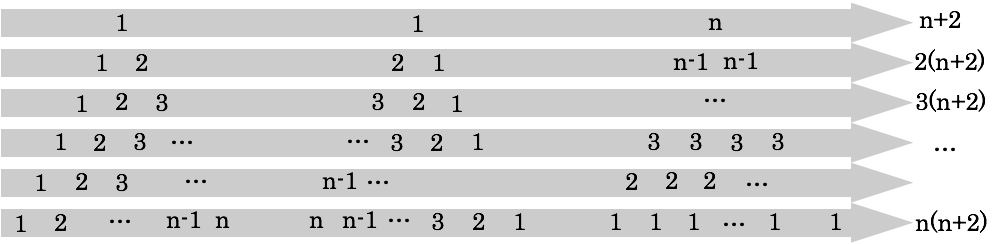
\includegraphics[scale=0.32]{FiguresArithmetic/appTetrahedral4}
        \caption{Detail of the computation of the invariant.}
        \label{fig:Tetrahedral4}
\end{center}
\end{figure}
Sum up the numbers in each row in Fig.~\ref{fig:Tetrahedral4}.
\begin{itemize}
\item 
The sum over the first row is equal to $1+1+n = n+2$.
\item
The second one is equal to $3 + 3 + 2.(n-1) = 2(n+2)$. 
\item
Let us sum up the elements in row $k$: 

$\Delta_k + \Delta_k + k(n-k+1)  = k(k+1) + kn-k^2+k = k(n+2)$.
\end{itemize}
$= \frac{1}{4}.\Theta_n.(n+3)$

The global sum is equal to $n+2$ times $(1+2+...+n)$.

Finally, $3 \Theta_n = (n+2) \Delta_n$
\medskip

\noindent \fbox{
\begin{minipage}{0.96\textwidth}
{\bf Explanatory note}.

\noindent \textit{Summary.} 
We proved the following results:
\begin{itemize}
\item $Id_n = 1+1+ ... +1 = n$
\item $\Delta_n = 1+2+3+ ... +n = \frac{1}{2}.Id_n.(n+1) = = \frac{n.(n+1)}{2}$
\item $\Theta_n = \Delta_1 + \Delta_2 + ... + \Delta_n = \frac{1}{3} .\Delta_n.(n+2) = \frac{1}{3}.\Delta_n.(n+2) = \frac{n.(n+1).(n+2)}{3!}$
\end{itemize}

Computing $\Theta_n$ corresponds to the third \textit{dimension}.
The idea of taking three copies of the triangles with rotating directions is natural
as the extension of the idea of taking two copies of the n integers (second dimension).
The dimension $1$ is simply to take one copy.  
\end{minipage}
}


%%%%%%%%%%%%%%%%%%%%
\section{$\oplus$ Pentahedral numbers}

As the previous results show some regularities, a natural question is: \textit{can we go further following the same pattern for computing 
$ \sum_{k=1}^{n} \Theta_k$?}
\medskip

Looking at the previous dimensions, the expected expression is:

$\Pi_n = \Theta_1 + \Theta_2 + ... + \Theta_n = \frac{1}{4}.\Theta_n.(n+3) = \frac{n.(n+1).(n+2).(n+3)}{4!} $

Again, it is possible to prove this expression by direct arithmetic manipulations
(replacing $\Theta_k$ by their expressions). 
It is not so easy to extend the previous construction, however, we know that there are $4$ copies of $\theta_n$ to consider.
Let organize three of them within the same triangular pattern in Fig.~\ref{fig:Tetrahedral6}.
\begin{figure}[h]
\begin{center}
        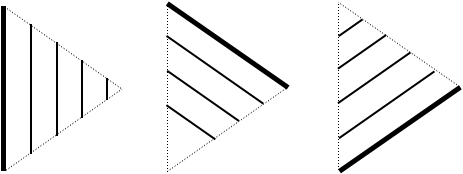
\includegraphics[scale=0.35]{FiguresArithmetic/appTetrahedral6}
        \caption{Computing $\Pi_n$: The three basic triangle patterns (solid lines represent integers with the same value).}
        \label{fig:Tetrahedral6}
\end{center}
\end{figure}
As each element is a $\Theta_k$, let decompose them again as in Fig.~\ref{fig:Tetrahedral7} for $n=4$.
\begin{figure}[h]
\begin{center}
        \includegraphics[scale=0.36]{FiguresArithmetic/appTetrahedral7}
        \caption{Computing $\Pi_n$: Organizing the three basic triangle patterns (for $n=4$).}
        \label{fig:Tetrahedral7}
\end{center}
\end{figure}
Let us add the remaining $\Theta_n$.
As for the previous lower dimension, summing up within each row leads to an invariant as shown in Fig.~\ref{fig:Tetrahedral5}.
\begin{figure}[h]
\begin{center}
        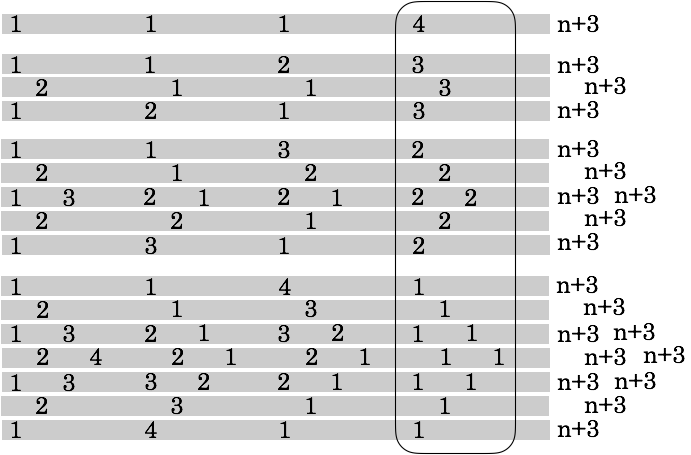
\includegraphics[scale=0.36]{FiguresArithmetic/appTetrahedral5}
        \caption{Add the last fourth copy of $\Theta_n$ and sum up the rows. The sum of elements of the last columns gives the result $\Theta.(n+3)$.}
        \label{fig:Tetrahedral5}
\end{center}
\end{figure}
The final result is easy to obtain:
\begin{itemize}
\item 
The sum over the first row is equal to $n+3$.
\item
The sum in the second series of rows is equal to $3.(n+3)$. 
\item
The sum of all the elements in the $k$th series of rows is equal to
$\Delta_k.(n+3)$.
\end{itemize}
$4.\Pi_n = (n+3) \sum_{k=1}^{n} \Delta_k = \Theta_n.(n+3)$


\subsection{Going further?}

Are you able to consider the challenge of going one step further?

We expect the sum of pentatonal numbers to be equal to:

$\frac{1}{5}.\Pi_n.(n+4) = \frac{n.(n+1).(n+2).(n+3).(n+4)}{5!}$


%%%%%%%%%%%%%%%%%%%%%%%%%%%%%%%%%%%%%%%%%%%%%%%%%%%%%%%%%%%%%%%

\section{Josephus' problem}


\subsection{description}

The problem studied in this section comes from the book \textit{R\'ecr\'eations math\'ematiques} of Edouard Lucas {\Denis put complete ref here and check the source...}.
He described this problem as an old story reported by Flavius Josephus during the Jewish-Roman war 
in the first century. 
The legend reports that Flavius was among a band of 41 rebels trapped in a cave by the roman army. Preferring suicide to capture, the
rebels decided to form a circle and proceeding around to kill every second remaining person until no one was left.
As Josephus did not want to die and had some skills in Mathematics, he quickly calculated
where he should stand in the circle in order to stay alive at the end of the process.
\medskip

The problem is formally described as follows.
 
Given $n$ successive numbers distributed along a circle.
The problem is to determine the \textit{survival number} (denoted by $J(n)$)
in the process of removing every second remaining number starting from $1$ (see figure~\ref{fig:josephus12step1}).
\begin{figure}[h]
\begin{center}
        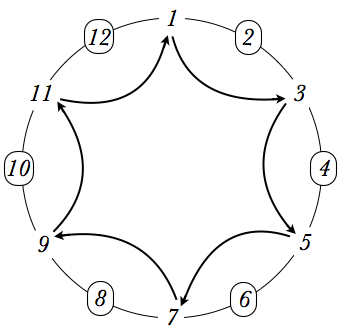
\includegraphics[scale=0.4]{FiguresMaths/josephus12step1}
        \caption{First round of the Josephus' cancellation process (for $n=12$).
        The $n$ first integers are spread over a circle, the integers in boxes are those that are removed.}
        \label{fig:josephus12step1}
\end{center}
\end{figure}


In particular, we are interested in knowing if there exists a \textit{closed formula}.
Guessing the answer is not straightforward. 
We need to better understand the progression by analyzing several cases (particular values of $n$).
\medskip

\begin{prop}
$J(n)$ is odd
\end{prop}

\begin{proof}
This is straightforward since the first tour removes all even numbers!
See figure~\ref{fig:josephus12step1}. 
\end{proof}
\medskip

\noindent
We called \textit{round}, the set of elementary steps to come back at the initial position in the circle. 
Starting at $1$, the first round is completed after $\lceil \frac{n}{2} \rceil$ steps. 
Then, again half of the of the remaining numbers are removed in the second round and so on.
Notice that the $1$ may be cancelled. In this case, the next step will start at the smallest remaining one.

How many rounds do we have for determining $J(n)$?
If $N$ denotes this number, it verifies
$\Sigma_{i=1}^{i=N} \frac{1}{2^i} = 1$.
\medskip

\begin{prop}. (even numbers)
$J(2n) = 2J(n)-1$ 
\end{prop}

\begin{figure}[h]
\begin{center}
        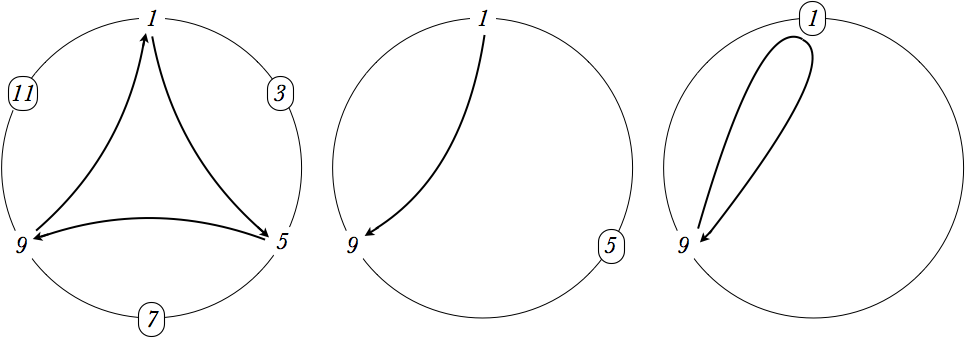
\includegraphics[scale=0.35]{FiguresMaths/josephus12LastSteps}
        \caption{Last rounds of the Josephus' cancellation process ($n=12$).}
        \label{fig:josephus12step2}
\end{center}
\end{figure}

{\begin{proof}
This is a simple generalization of the previous proposition.
If $n$ is even, the first round corresponds simply to come back to the original circle where one half of the points have been removed. 
\end{proof}

From this, we deduce $J(2^m)=1$ for all $m$.
\medskip

Let us turn to odd numbers.
\begin{figure}[h]
\begin{center}
        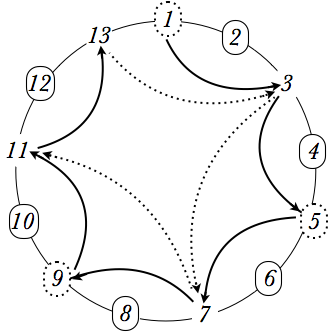
\includegraphics[scale=0.4]{FiguresMaths/josephus13}
        \caption{The two first rounds of the Josephus' cancellation process (for $n=13$).
        The first one is is depicted by solid lines, the second one is with dotted lines.}
        \label{fig:josephus13}
\end{center}
\end{figure}
%Figure~\ref{fig:josephus13} depicted an example for $n=13$. 
\medskip

\begin{prop} (odd numbers)
$J(2n+1) = 2J(n)+1$ 
\end{prop}

We can compute easily the first ranks.
It turns out that the progression is composed of grouped terms starting at each power of $2$. 
{\Denis should we detail here for instance up to n=20?}

{\Denis 1 -- 1 2 -- 1.2 3 4 -- 1 2 3 4 5 6 7  8 -- 1  2  3 4 ...}

Let $n=2^m+k$, the rule within each group $m$ is to start at $1$ and increase by $2$ the successive numbers
($0 \leq k < 2^m$).
Let prove it by recurrence on $n$.
\medskip

\begin{prop}
$J(2^m+k) = 2k+1$ 
\end{prop}

\begin{proof}
\begin{itemize}
\item {\bf Basis.} 
$n=1$, thus $m=0$, $k=0$ and $J(1) = 2^0+0 = 1$
\item {\bf Induction step.} 
Suppose the formula holds for any integer lower than $n=2^m+k$. 
Since there are two expressions for $J(.)$, we distinguish the cases whether $k$ is even or it is odd:
\begin{itemize}
\item If $k$ is even, then, $2^m+k$ is even, and we can write:

$J(2^m+k) = 2J(2^{m-1}+\frac{k}{2})-1$

by induction hypothesis, $J(2^{m-1} +\frac{k}{2}) = 2\frac{k}{2} +1 = k+1$

Thus, $J(2^m+k) = 2(k+1) -1 = 2k+1$.

\item If $k$ is odd, the proof is similar:

$J(2^m+k) = 2J(2^{m-1}+\lfloor \frac{k}{2} \rfloor)+1 = 2\lfloor \frac{k}{2} \rfloor +1 = 2k+1$.

\end{itemize}
\end{itemize}
\end{proof}

\subsection{Coding}

We can even go one step further with this problem by remarking that powers of $2$ play an important role.
Let us use the radix $2$ representation of $n$ and $J(n)$:

$n = \sum_{j=0}^{j=m} b_j.2^j = b_m.2^m + b_{m-1}.2^{m-1} + ... + b_1.2 + b_0$

$n = (1 b_{m-1} ... b_1 b_0)_2$ since by definition of $m$ $b_m=1$ 

$k = (0 b_{m-1} ... b_1 b_0)_2$ since $k < 2^m$

Thus, using the closed formula for $J(n)$:

$J(n) = (b_{m-1} ... b_0 b_m)_2$.

The pictorial interpretation of this coding is given in Fig.~\ref{fig:josephusCoding} for $n=43$.
\begin{figure}[h]
\begin{center}
        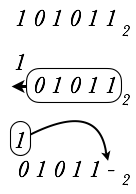
\includegraphics[scale=0.4]{FiguresMaths/josephusCoding}
        \caption{Process for obtaing the josephus' number of $n=43$.}
        \label{fig:josephusCoding}
\end{center}
\end{figure}

In other words, the solution is obtained by a simple shift of the binary representation of $n$.

We showed here how mathematics are powerful: the analysis leads to an expression that can be obtained in 2 simple operations!


